\begin{FlowRevisionText}
\FloatBarrier
\par\medskip
\noindent\textbf{تکرار مطالعه با وزن جدید اپراتور جریان.}\par\smallskip
اپراتور بازآموزی‌شده با وزن گام $314000$ در برازش استفاده شد.
هر نه پروفایل و مسیرهای مشاهده‌شده با آزمون قبلی مشترک بودند.
رهاسازی‌ها شامل مکان، تندی و جهت‌های متنوع و تصادفی بودند.
تعداد ذرات از دو شروع شد و تطبیقی افزایش یافت.
نمودارها پنج یا شش برازش واقعی را نشان می‌دهند.
منحنی نقطه‌چین فقط برای تعدادهای مشترکِ آزموده‌شده رسم شده است.
آستانهٔ خطای پروفایل $5\%$ و سقف پیمایش $24$ ذره بود.
برای توقف زودهنگام، چند مرحلهٔ بیشتر به نمایش افزوده شد.
حقیقت ورودی برای ارزیابی و انتخاب تعداد استفاده شد.
پارامترهای اولیهٔ ذرات در برازش معلوم بودند.

شکل~\ref{fig:soap-particle-beta5} بازسازی ورودی بتای باریک را نشان می‌دهد.
خطای مرحلهٔ پایانی با $21$ ذره، $2.76\%$ بود.
نخستین تعداد موفق آزموده‌شده $17$ ذره بود.
\begin{figure}[htbp]
\centering
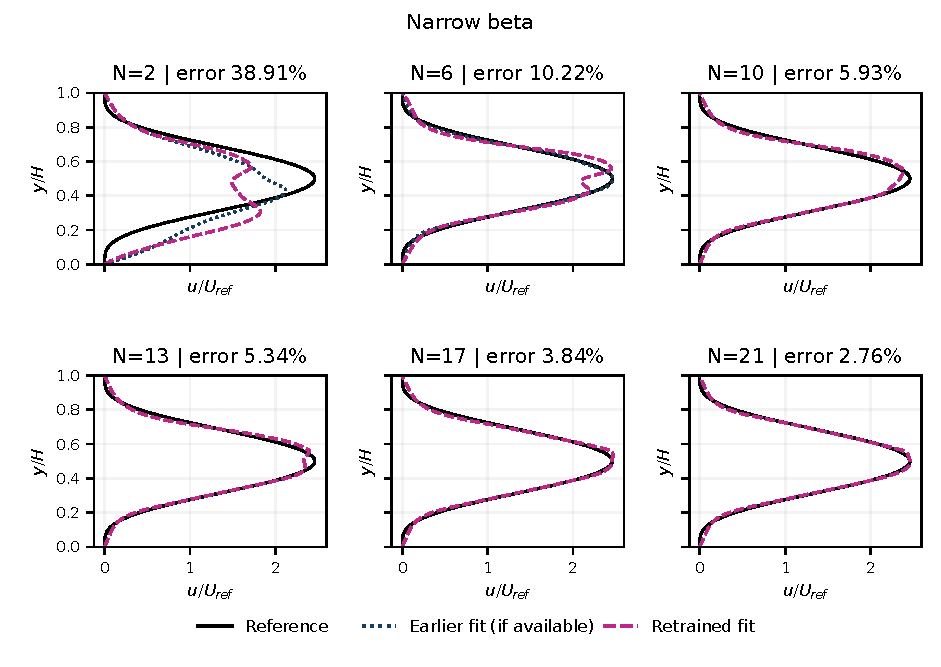
\includegraphics[width=\textwidth]{New_Adaptive_Particle_Results/soap_314k/figures/beta5.pdf}
\caption[بازسازی ورودی بتای باریک با وزن جدید و افزایش تعداد ذرات.]{\FlowRevision{بازسازی ورودی بتای باریک با وزن جدید و افزایش تعداد ذرات.}}
\label{fig:soap-particle-beta5}
\end{figure}
\FloatBarrier
شکل~\ref{fig:soap-particle-skew_b3} بازسازی ورودی نامتقارن را نشان می‌دهد.
خطای مرحلهٔ پایانی با $21$ ذره، $3.81\%$ بود.
\begin{figure}[htbp]
\centering
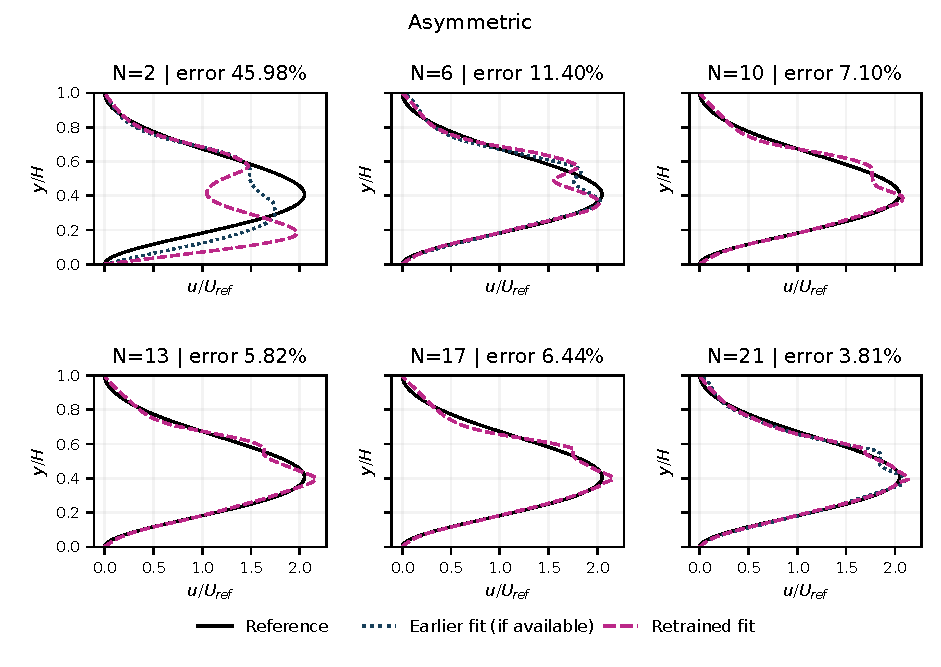
\includegraphics[width=\textwidth]{New_Adaptive_Particle_Results/soap_314k/figures/skew_b3.pdf}
\caption[بازسازی ورودی نامتقارن با وزن جدید و افزایش تعداد ذرات.]{\FlowRevision{بازسازی ورودی نامتقارن با وزن جدید و افزایش تعداد ذرات.}}
\label{fig:soap-particle-skew_b3}
\end{figure}
\FloatBarrier
شکل~\ref{fig:soap-particle-flat30} بازسازی ورودی تقریباً تخت را نشان می‌دهد.
خطای مرحلهٔ پایانی با $24$ ذره، $5.16\%$ بود.
در تعدادهای آزموده‌شده، خطا به آستانهٔ پنج درصد نرسید.
\begin{figure}[htbp]
\centering
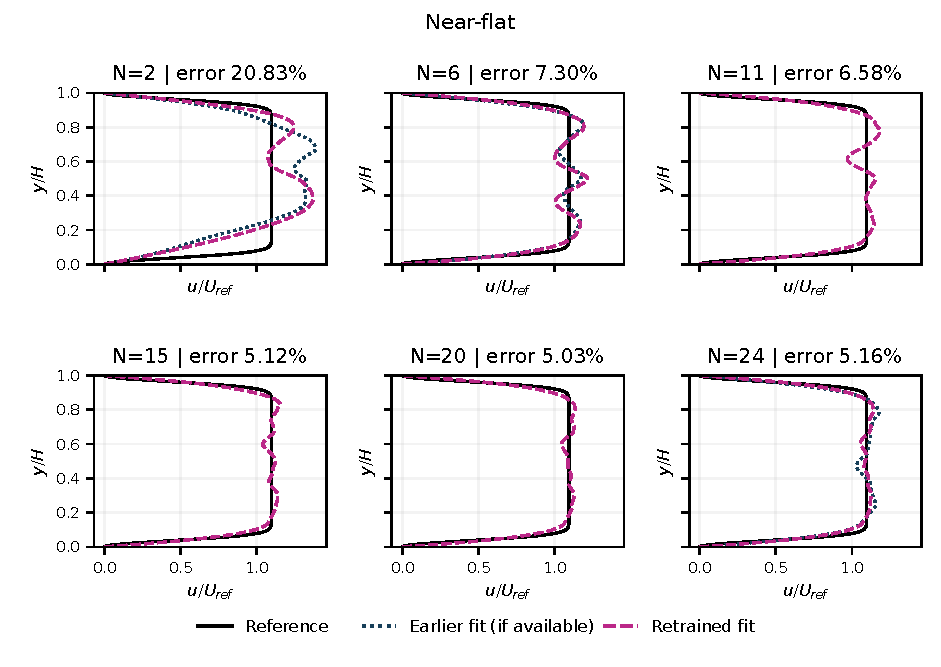
\includegraphics[width=\textwidth]{New_Adaptive_Particle_Results/soap_314k/figures/flat30.pdf}
\caption[بازسازی ورودی تقریباً تخت با وزن جدید و افزایش تعداد ذرات.]{\FlowRevision{بازسازی ورودی تقریباً تخت با وزن جدید و افزایش تعداد ذرات.}}
\label{fig:soap-particle-flat30}
\end{figure}
\FloatBarrier
شکل~\ref{fig:soap-particle-twin_b3_r30} بازسازی ورودی دوقله‌ای را نشان می‌دهد.
خطای مرحلهٔ پایانی با $6$ ذره، $4.51\%$ بود.
\begin{figure}[htbp]
\centering
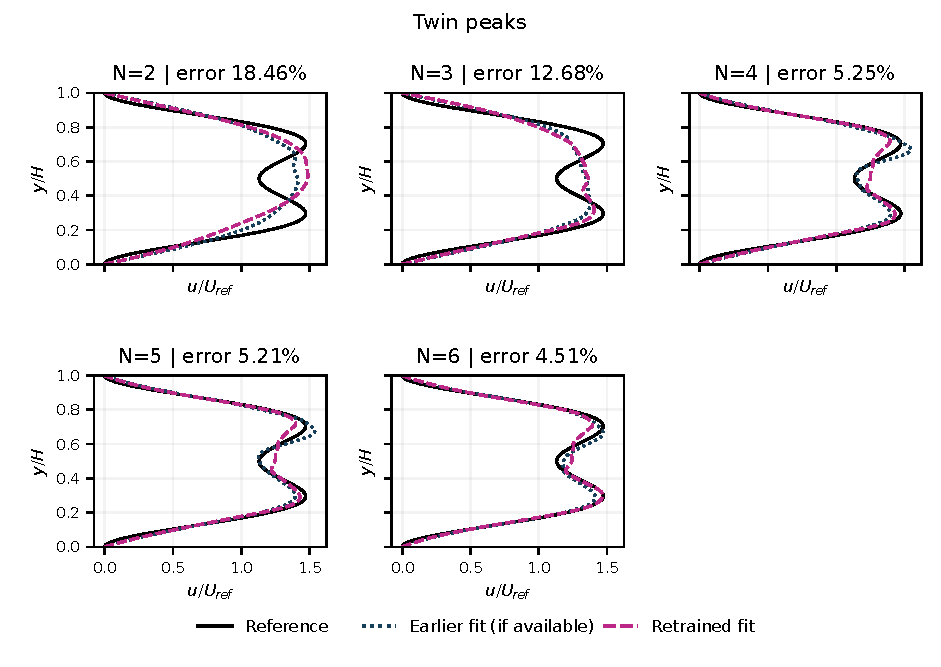
\includegraphics[width=\textwidth]{New_Adaptive_Particle_Results/soap_314k/figures/twin_b3_r30.pdf}
\caption[بازسازی ورودی دوقله‌ای با وزن جدید و افزایش تعداد ذرات.]{\FlowRevision{بازسازی ورودی دوقله‌ای با وزن جدید و افزایش تعداد ذرات.}}
\label{fig:soap-particle-twin_b3_r30}
\end{figure}
\FloatBarrier
شکل~\ref{fig:soap-particle-shoulder} بازسازی ورودی شانه‌دار را نشان می‌دهد.
خطای مرحلهٔ پایانی با $24$ ذره، $5.37\%$ بود.
در تعدادهای آزموده‌شده، خطا به آستانهٔ پنج درصد نرسید.
\begin{figure}[htbp]
\centering
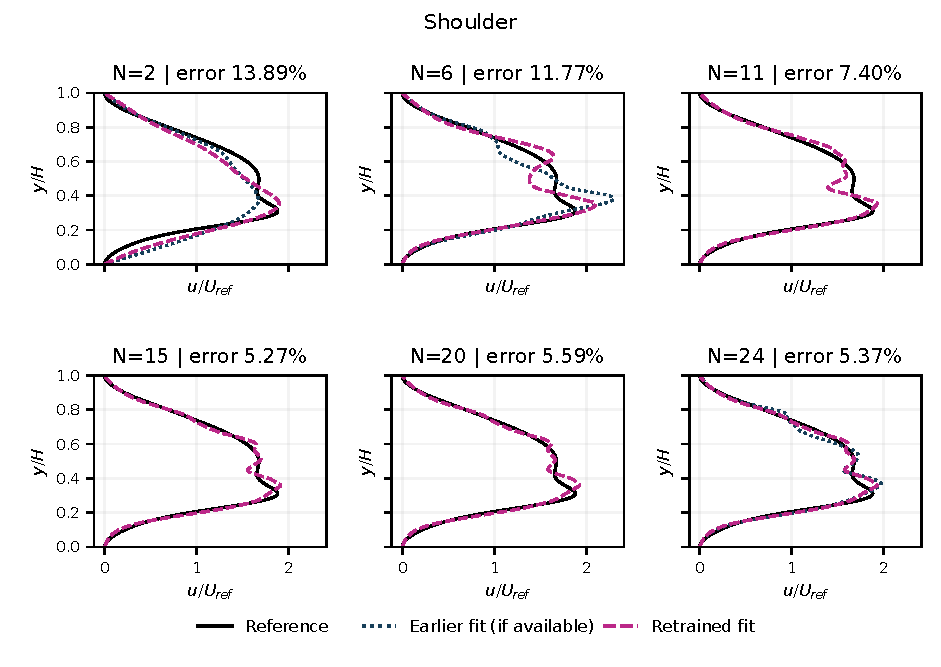
\includegraphics[width=\textwidth]{New_Adaptive_Particle_Results/soap_314k/figures/shoulder.pdf}
\caption[بازسازی ورودی شانه‌دار با وزن جدید و افزایش تعداد ذرات.]{\FlowRevision{بازسازی ورودی شانه‌دار با وزن جدید و افزایش تعداد ذرات.}}
\label{fig:soap-particle-shoulder}
\end{figure}
\FloatBarrier
شکل~\ref{fig:soap-particle-mixed} بازسازی ورودی چندمقیاسی را نشان می‌دهد.
خطای مرحلهٔ پایانی با $24$ ذره، $7.03\%$ بود.
در تعدادهای آزموده‌شده، خطا به آستانهٔ پنج درصد نرسید.
\begin{figure}[htbp]
\centering
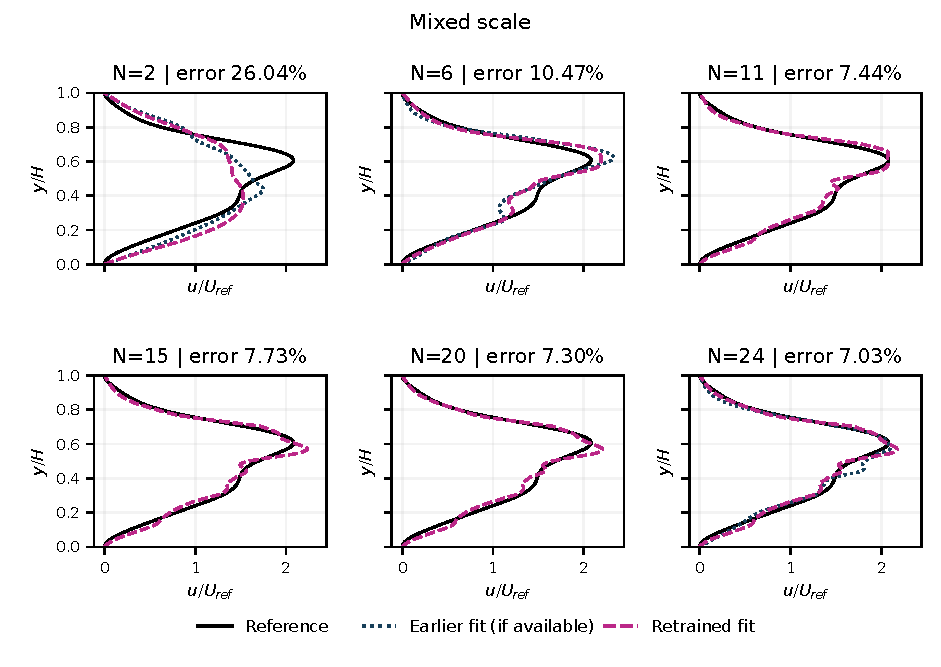
\includegraphics[width=\textwidth]{New_Adaptive_Particle_Results/soap_314k/figures/mixed.pdf}
\caption[بازسازی ورودی چندمقیاسی با وزن جدید و افزایش تعداد ذرات.]{\FlowRevision{بازسازی ورودی چندمقیاسی با وزن جدید و افزایش تعداد ذرات.}}
\label{fig:soap-particle-mixed}
\end{figure}
\FloatBarrier
شکل~\ref{fig:soap-particle-waves3_r30} بازسازی ورودی سه‌نوسانی را نشان می‌دهد.
خطای مرحلهٔ پایانی با $6$ ذره، $5.77\%$ بود.
نخستین تعداد موفق آزموده‌شده $4$ ذره بود.
\begin{figure}[htbp]
\centering
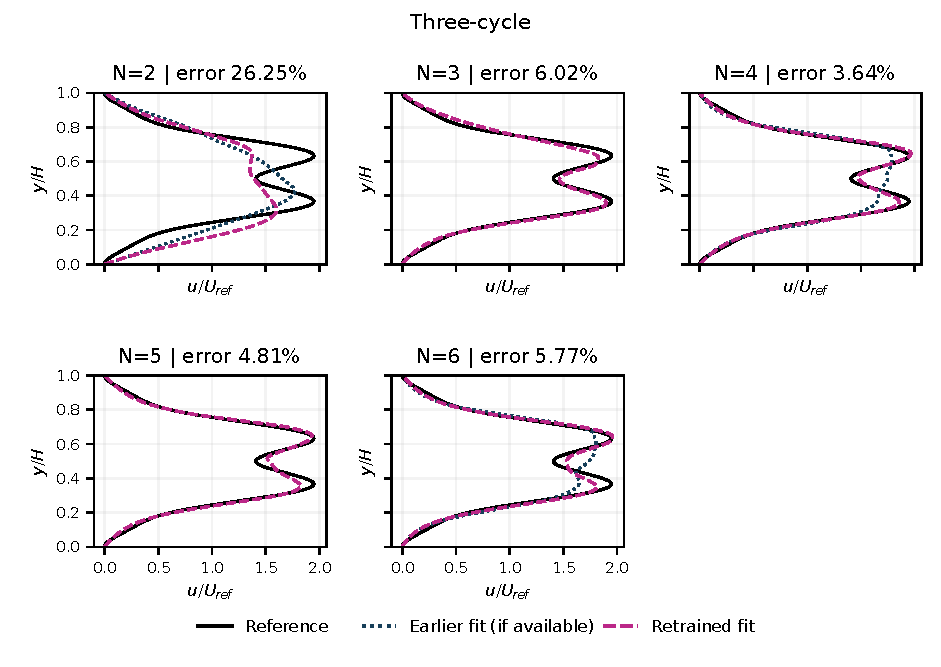
\includegraphics[width=\textwidth]{New_Adaptive_Particle_Results/soap_314k/figures/waves3_r30.pdf}
\caption[بازسازی ورودی سه‌نوسانی با وزن جدید و افزایش تعداد ذرات.]{\FlowRevision{بازسازی ورودی سه‌نوسانی با وزن جدید و افزایش تعداد ذرات.}}
\label{fig:soap-particle-waves3_r30}
\end{figure}
\FloatBarrier
شکل~\ref{fig:soap-particle-lobes4_r30} بازسازی ورودی چهارنوسانی را نشان می‌دهد.
خطای مرحلهٔ پایانی با $24$ ذره، $18.17\%$ بود.
در تعدادهای آزموده‌شده، خطا به آستانهٔ پنج درصد نرسید.
\begin{figure}[htbp]
\centering
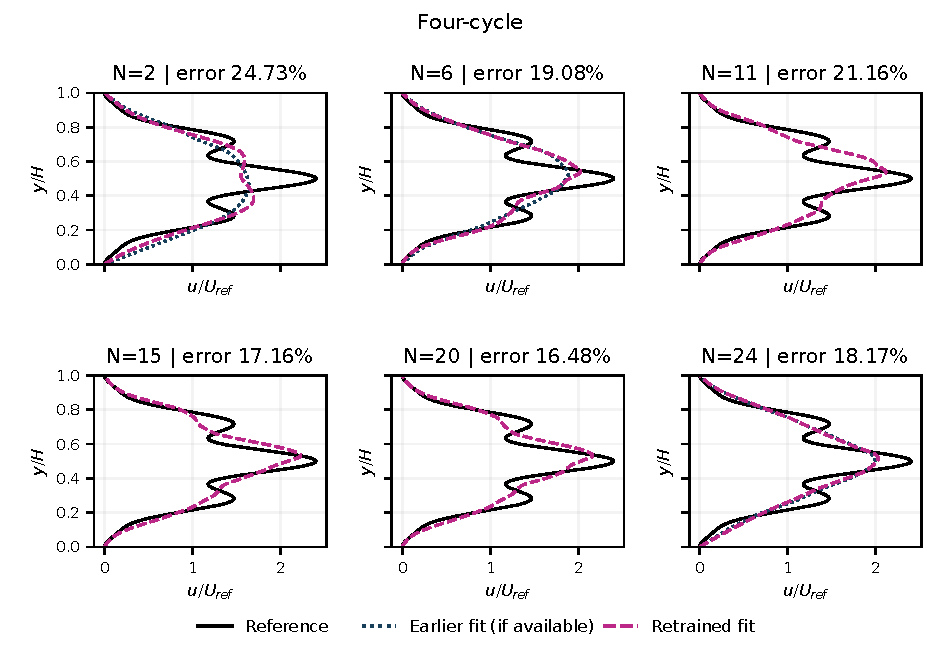
\includegraphics[width=\textwidth]{New_Adaptive_Particle_Results/soap_314k/figures/lobes4_r30.pdf}
\caption[بازسازی ورودی چهارنوسانی با وزن جدید و افزایش تعداد ذرات.]{\FlowRevision{بازسازی ورودی چهارنوسانی با وزن جدید و افزایش تعداد ذرات.}}
\label{fig:soap-particle-lobes4_r30}
\end{figure}
\FloatBarrier
شکل~\ref{fig:soap-particle-nine30} بازسازی ورودی نه‌نوسانی را نشان می‌دهد.
خطای مرحلهٔ پایانی با $15$ ذره، $38.90\%$ بود.
در تعدادهای آزموده‌شده، خطا به آستانهٔ پنج درصد نرسید.
\begin{figure}[htbp]
\centering
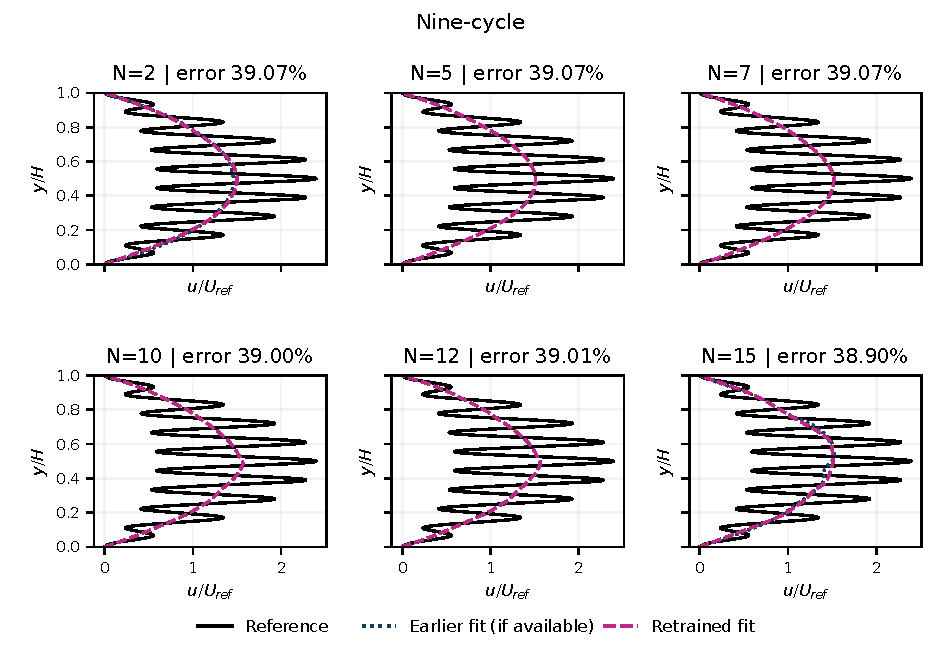
\includegraphics[width=\textwidth]{New_Adaptive_Particle_Results/soap_314k/figures/nine30.pdf}
\caption[بازسازی ورودی نه‌نوسانی با وزن جدید و افزایش تعداد ذرات.]{\FlowRevision{بازسازی ورودی نه‌نوسانی با وزن جدید و افزایش تعداد ذرات.}}
\label{fig:soap-particle-nine30}
\end{figure}
\FloatBarrier
\par\medskip
\noindent\textbf{تکرار آزمون رهاسازی نزدیک ورودی.}\par\smallskip
شرایط رهاسازی و زمان‌های مشاهده با آزمایش هدفمند قبلی مشترک بودند.
ضریب زبری و سقف تکرار همان تنظیمات آزمون هدفمند قبلی بودند.
شکل~\ref{fig:soap-particle-near} روند بازسازی پروفایل نه‌نوسانی را نشان می‌دهد.
خطای مرحلهٔ پایانی با $48$ ذره، $6.20\%$ بود.
در ادامه، رهاسازی‌های بیشتری با همان الگوی نزدیک ورودی افزوده شدند.
مسیرهای ۲۴ ذرهٔ نخست در این گسترش یکسان ماندند.
\begin{figure}[htbp]
\centering
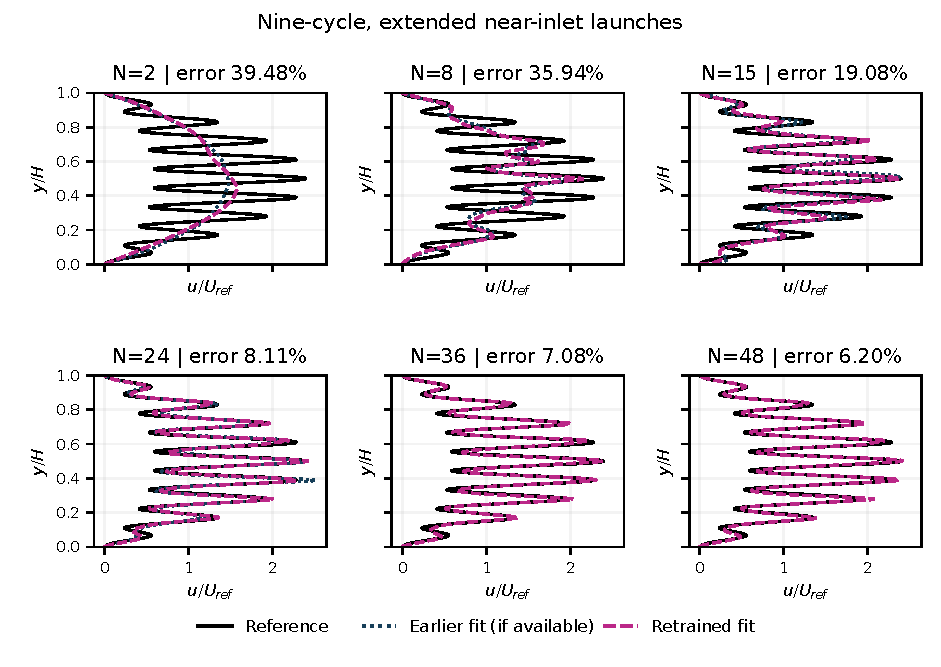
\includegraphics[width=\textwidth]{New_Adaptive_Particle_Results/soap_314k_near_extended/figures/nine30.pdf}
\caption[بازسازی ورودی نه‌نوسانی با رهاسازی هدفمند و وزن جدید.]{\FlowRevision{بازسازی ورودی نه‌نوسانی با رهاسازی هدفمند و وزن جدید.}}
\label{fig:soap-particle-near}
\end{figure}
\FloatBarrier
\end{FlowRevisionText}
